\documentclass{beamer}
\usepackage[utf8]{inputenc}
\usepackage{graphicx}
\usepackage{tikz}
\usetikzlibrary{arrows,shapes,positioning}
\usepackage[center]{caption}
\usepackage[english]{babel}

%---------------------------------------------
% Font packages
%---------------------------------------------
\usepackage{lmodern}
% \usepackage{concmath}
% \usepackage{cmbright}
% \usepackage{kpfonts}
% \usepackage[adobe-utopia]{mathdesign}
%\usepackage{fouriernc}
\usepackage[T1]{fontenc}

%---------------------------------------------
% Math environment packages & command
%---------------------------------------------
\usepackage{amsmath}
\usepackage{amssymb}
\usepackage{array}
% \usepackage{mathrsfs}
\usepackage{array}
% \def\sgn{\mathop{\rm sgn}\nolimits} 
% \usepackage{bbm}


\usetheme{CambridgeUS}
%\useoutertheme{sidebar} %: Ligne à commenter dans un premier temps, et à décommentez dans un second temps.

%---------------------------------------------
% Opening
%---------------------------------------------
\title{\textsc{Micro Management in Real Time Strategy Games}}
%\author{Björn \textsc{Holm}, Kilian \textsc{Demeulemeester} \\ \texttt{\{bjh,kiliande\}@kth.se}}
\author{Björn \textsc{Holm}
    \and
Kilian \textsc{Demeulemeester}}
\date{\today}

%---------------------------------------------
% Numerotation Handling
%---------------------------------------------
 %\setcounter{section}{3}

 %---------------------------------------------
% Bibliography package
%---------------------------------------------
\usepackage{url}
\hypersetup{urlcolor=black}
\usepackage{breakurl}

%---------------------------------------------
% Item package option 
%---------------------------------------------
\newenvironment{shortitem}{
    \begin{itemize}
        \setlength{\item[-]sep}{0pt}
        \setlength{\parskip}{0pt}
        \setlength{\parsep}{0pt}
    }{\end{itemize}}



\begin{document}

\begin{frame}
    \maketitle
\end{frame}

\section{Scope}

\begin{frame}
\frametitle{Scope}
\begin{itemize}
\item[-] Micro-management only
\item[-] 1 vs 1
\item[-] Same number of units
\item[-] Destroy all enemy units
\item[-] Maximize the number of survivors
\item[-] Full knowledge of game state
\end{itemize}
\end{frame}

\section{Model \& Architecture}

\begin{frame}
\frametitle{Model \& Architecture}
\begin{center}
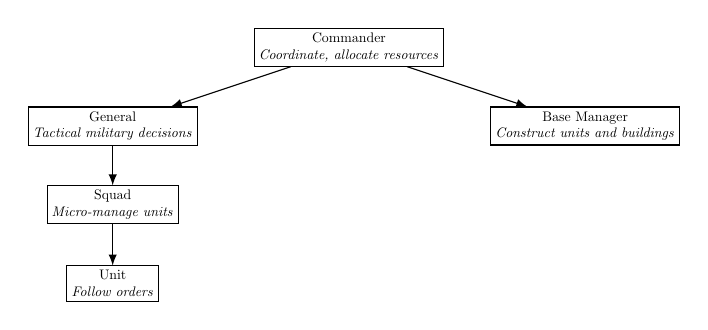
\begin{tikzpicture}[node distance = 1 cm]
    \tikzstyle{quadri}=[rectangle,draw, align=center, scale=0.5]
    \tikzstyle{link}=[->,thin,>=latex]
    \node[quadri] (commander) at (0,2) {Commander \\ \emph{Coordinate, allocate resources}};
    \node[quadri] (general) at (-3,1) {General \\ \emph{Tactical military decisions}};
    \node[quadri] (squad) at (-3,0) {Squad \\ \emph{Micro-manage units}};
    \node[quadri] (unit) at (-3,-1) {Unit \\ \emph{Follow orders}};
    \node[quadri] (basemanager) at (3,1) {Base Manager \\ \emph{Construct units and buildings}};
    \draw[link] (commander)--(general);
    \draw[link] (general)--(squad);
    \draw[link] (squad)--(unit);
    \draw[link] (commander)--(basemanager);
\end{tikzpicture}
\end{center}
\end{frame}

\section{Our bots}

\begin{frame}
\frametitle{Our bots}
\begin{itemize}
\item[-] \texttt{Attack Closest:} Every unit attack their closest opponent.
\item[-] \texttt{Attack Closest Lethal:} Every unit attack the closest opponent that will not die soon (\emph{i.e.} the amount of damage attributed to this unit is not already enough to kill him soon).
\item[-] \texttt{Kiting:} Every unit attacks their closest opponent applying a kiting strategy.
\item[-] \texttt{Searching:} A searching algorithm trying to find the best option for moving or which opponent to attacking in any situation.

\end{itemize}
\end{frame}

\section{Kiting}


\begin{frame}
\frametitle{Kiting}
\begin{center}
    \begin{figure}
        \centering
        \includegraphics[height=5cm]{fig.ps}
        \caption{Influence matrix created by a group of 6 units \\ 
        Lighter blue means bigger value}
        \label{influenceMatrix}
    \end{figure}
\end{center}
\end{frame}


\begin{frame}
\frametitle{Kiting}
\begin{center}
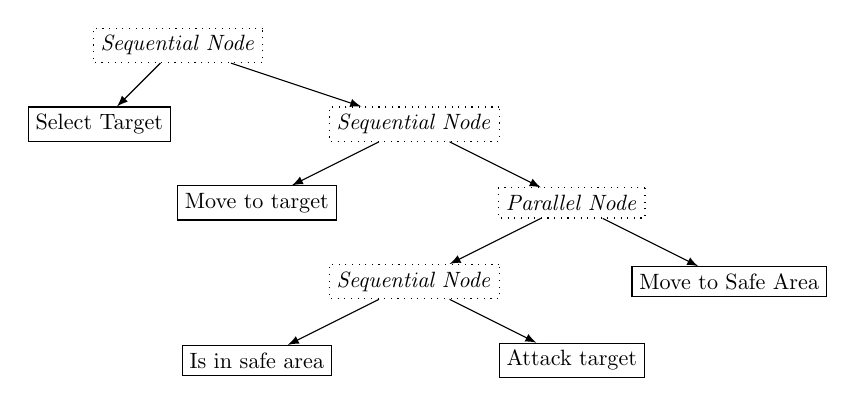
\begin{tikzpicture}[node distance = 1 cm]
    \tikzstyle{leaf}=[rectangle, align=center, scale=0.8, draw]
    \tikzstyle{node}=[rectangle,dotted, align=center, scale=0.8, draw]
    \tikzstyle{link}=[->,thin,>=latex]
    \node[node] (start) at (1,4) {\emph{Sequential Node}};

    \node[leaf] (target) at (0,3) {Select Target};
    \node[node] (seqNode) at (4,3) {\emph{Sequential Node}};

    \node[leaf] (leafMove) at (2,2) {Move to target};
    \node[node] (paraAttack) at (6,2) {\emph{Parallel Node}};

    \node[node] (attackNode) at (4,1) {\emph{Sequential Node}};
    \node[leaf] (moveSafe) at (8,1) {Move to Safe Area};

    \node[leaf] (isSafe) at (2,0) {Is in safe area};
    \node[leaf] (attack) at (6,0) {Attack target};

    \draw[link] (start)--(target);
    \draw[link] (start)--(seqNode);

    \draw[link] (seqNode)--(leafMove);
    \draw[link] (seqNode)--(paraAttack);

    \draw[link] (paraAttack)--(attackNode);
    \draw[link] (paraAttack)--(moveSafe);

    \draw[link] (attackNode)--(attack);
    \draw[link] (attackNode)--(isSafe);
\end{tikzpicture}
\end{center}
\end{frame}


\section{Search}

\begin{frame}
\frametitle{Search}
The marine attack action
\begin{center}
\begin{tabular}{ r | p{3,5cm} }
Frame offset & Effect \\
\hline
0 & marine may not move \\
1 & damage is applied to target \\
6 & marine may move again \\
14-17 & marine may attack again\footnotemark
\end{tabular}
\footnotetext{The exact number is randomed every attack.}
\end{center}
\end{frame}

\begin{frame}
\frametitle{Search}
The firebat attack action
\begin{center}
\begin{tabular}{ r | p{3,5cm} }
Frame offset & Effect \\
\hline
0 & firebat may not move \\
5 & half of the damage is applied to target \\
6 & if the firebat is still alive, the other half of the damage is applied to the target as well \\
10 & the firebat may move again \\
21-24 & the firebat may attack again
\end{tabular}
\end{center}
\end{frame}

\begin{frame}
\frametitle{Search}
Monte Carlo Tree Search algorithm

\begin{center}
\begin{tabular}{ | l | p{3,5cm} | }
\hline
\multicolumn{2}{|c|}{\emph{GameState}} \\
\hline
units		& all the units with their positions, health, and internal states \\
effects	& all the pending effects to be applied to the GameState at a future frame. \\
\hline
\end{tabular}
\end{center}
\end{frame}

\section{Results}

\begin{frame}
\frametitle{Results}
\begin{itemize}
\item[-] \texttt{Attack Closest:} Defeated
\item[-] \texttt{Attack Closest Lethal:} almost 100\% -- show real cooperation behaviors
\item[-] \texttt{Kiting:} almost 100\% -- some bugs
\item[-] \texttt{Searching:} Not implemented
\end{itemize}
\end{frame}

\section{Future work}

\begin{frame}
\frametitle{Future work}
Potential topics:
\begin{itemize}
\item[-] Implement search bot
\item[-] Handle 3 types of units ($A > B > C > A \dots$)
\item[-] Add ressources generation at constant rate \& produce units
\item[-] Kill the king !
\end{itemize}
\end{frame}
\end{document}
